%This is the article LaTeX template for RSC journals
%Copyright The Royal Society of Chemistry 2010
% \usepackage{times}
% feel free not to use mathptmx if it causes difficulties
%eps figures can be used instead


\documentclass[8.5pt,twoside,twocolumn]{article}
%%%%%%%%%%%%%%%%%%%%%%%%%%%%%%%%%%%%%%%%%%%%%%%%%%%%%%%%%%%%%%%%%%%%%%%%%%%%%%%%%%%%%%%%%%%%%%%%%%%%%%%%%%%%%%%%%%%%%%%%%%%%%%%%%%%%%%%%%%%%%%%%%%%%%%%%%%%%%%%%%%%%%%%%%%%%%%%%%%%%%%%%%%%%%%%%%%%%%%%%%%%%%%%%%%%%%%%%%%%%%%%%%%%%%%%%%%%%%%%%%%%%%%%%%%%%
\usepackage{amssymb}
\usepackage{eurosym}
\usepackage[super,sort&compress,comma]{natbib}
\usepackage{mhchem}
\usepackage{times,mathptmx}
\usepackage{units}
\usepackage{sectsty}
\usepackage{balance}
\usepackage{graphicx}
\usepackage{epstopdf}
\usepackage{lastpage}
\usepackage[format=plain,justification=raggedright,singlelinecheck=false,font=small,labelfont=bf,labelsep=space]{caption}
\usepackage{fancyhdr}

%TCIDATA{OutputFilter=LATEX.DLL}
%TCIDATA{Version=5.50.0.2960}
%TCIDATA{<META NAME="SaveForMode" CONTENT="1">}
%TCIDATA{BibliographyScheme=BibTeX}
%TCIDATA{LastRevised=Sunday, August 10, 2014 15:18:51}
%TCIDATA{<META NAME="GraphicsSave" CONTENT="32">}

\oddsidemargin -1.2cm
\evensidemargin -1.2cm
\textwidth 18cm
\headheight 1.0in
\topmargin -3.5cm
\textheight 22cm

\input{tcilatex}

\begin{document}


\thispagestyle{plain} 
\fancypagestyle{plain}{
\renewcommand{\headrulewidth}{1pt}} \renewcommand{\thefootnote}{%
\fnsymbol{footnote}} 
\renewcommand\footnoterule{\vspace*{1pt}\hrule width
3.4in height 0.4pt \vspace*{5pt}} \setcounter{secnumdepth}{5}

\makeatletter

\renewcommand\@biblabel[1]{#1} \renewcommand\@makefntext[1]{\noindent%
\makebox[0pt][r]{\@thefnmark\,}#1} \makeatother
\renewcommand{\figurename}{\small{Fig.}~} \sectionfont{\large} %
\subsectionfont{\normalsize}

%\fancyfoot{} \fancyfoot[LO,RE]{\vspace{-7pt}%
%\includegraphics[height=9pt]{headers/LF}} \fancyfoot[CO]{\vspace{-7.2pt}%
%\hspace{12.2cm}\includegraphics{headers/RF}} \fancyfoot[CE]{\vspace{-7.5pt}%
%\hspace{-13.5cm}\includegraphics{headers/RF}} \fancyfoot[RO]{\footnotesize{%
%\sffamily{1--\pageref{LastPage} ~\textbar  \hspace{2pt}\thepage}}} 
%\fancyfoot[LE]{\footnotesize{\sffamily{\thepage~\textbar\hspace{3.45cm}
%1--\pageref{LastPage}}}} \fancyhead{} \renewcommand{\headrulewidth}{1pt} %
\renewcommand{\footrulewidth}{1pt} \setlength{\arrayrulewidth}{1pt} %
\setlength{\columnsep}{6.5mm} \setlength\bibsep{1pt}

\twocolumn[
  \begin{@twocolumnfalse}
\noindent\LARGE{\textbf{Ultrasoft elastomers near gel limit}}
\vspace{0.6cm}

\noindent\large{\textbf{Li-Heng Cai,\textit{$^{a,\dag}$} Thomas E. Kodger,\textit{$^{a,\dag}$} Jacqueline Flood,\textit{$^{a}$} and
David A. Weitz $^{\ast}$\textit{$^{a}$}}}


\vspace{0.6cm}

\noindent \normalsize{\textbf{Abstract:} Modulus of an elastomer near gel limit}
\vspace{0.5cm}
\end{@twocolumnfalse}
]

%Footnotes
%\footnotetext{%
%\dag ~Electronic Supplementary Information (ESI) available: [details of any
%supplementary information available should be included here]. See DOI:
%10.1039/b000000x/}

%Please use \dag to cite the ESI in the main text of the article.
%If you article does not have ESI please remove the the \dag symbol from the title and the above footnotetext.

\footnotetext{\textit{$^{a}$School of Engineering and Applied Sciences,
Harvard University, Cambridge, Massachusetts 02138, United States. $^{\dag}$%
These authors contributed to the work equally. $^{\ast}$Correspondence:
weitz@seas.harvard.edu}}

%additional addresses can be cited as above using the lower-case letters, c, d, e... If all authors are from the same address, no letter is required

%\footnotetext{%
%\ddag ~Additional footnotes to the title and authors can be included \emph{%
%e.g.}\ `Present address:' or `These authors contributed equally to this
%work' as above using the symbols: \ddag , \textsection, and \P . Please
%place the appropriate symbol next to the author's name and include a \texttt{%
%\TEXTsymbol{\backslash}footnotetext} entry in the the correct place in the
%list.}

\begin{figure}[h]
\centering
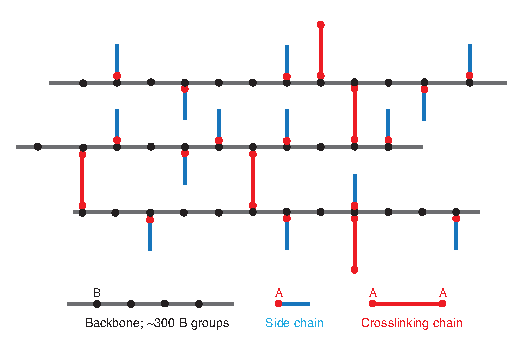
\includegraphics[scale=1]{figures/fig1_cartoon.eps}
\caption{\textbf{cartoon}}
\label{fig:illustration}
\end{figure}

\begin{figure}[h]
\centering
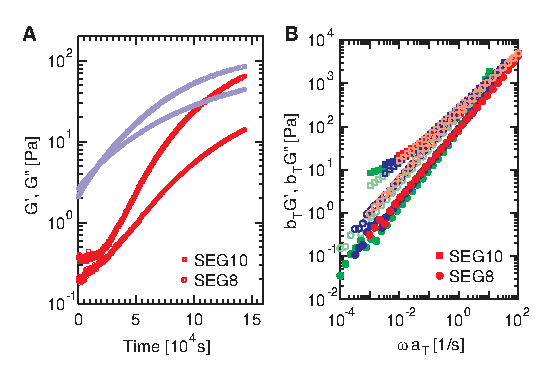
\includegraphics[scale=1]{figures/fig2.eps}
\caption{Determine the gel limit of soft PDMS elastomers by reducing the
number of ratio of backbone polymers and side chains. (A) Time-sweeps to
monitor the polymerization of samples with backbone polymer and side chains
of number ratios nbb:nsc=1:10 (SEG10) and nbb:nsc=1:8 (SEG8). (B) Frequency
dependence of the storage (G, filled symbols) and loss (G, empty symbols) of
different samples obtained by classical time-temperature superposition
shifts. The reference temperature is -20 oC and the measurements are
performed at -20oC (red), 20oC (blue) and 80oC (green). The shifting
parameters are the same for all samples: aT = 1/9.5 for 20 oC and 1/3 for 80
oC; bT = 253/T, in which T is the absolute temperature. }
\label{fig:11}
\end{figure}

\begin{figure}[h]
\centering
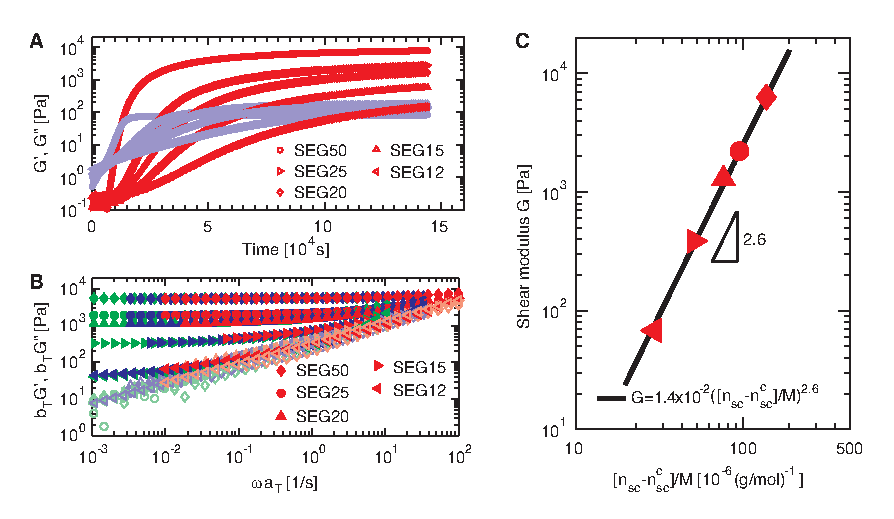
\includegraphics[scale=1]{figures/fig3.eps}
\caption{\textbf{cartoon}}
\label{fig:illustration}
\end{figure}

\begin{tabular}{cccccc}
&  &  &  &  &  \\ 
&  &  &  &  &  \\ 
&  &  &  &  &  \\ 
&  &  &  &  &  \\ 
&  &  &  &  & 
\end{tabular}

\textbf{Acknowledgment.} We acknowledge financial support from the National
Science Foundation under grants CHE-0911588, DMR-0907515, DMR-1121107,
DMR-1122483, and CBET-0609087, the National Institutes of Health under
grants R01HL077546 and P50HL107168, and Cystic Fibrosis Foundation under
grant RUBIN09XX0.

%The conclusions section should come at the end of article. For the reference
%section, the style file rsc.bst can be used to generate the correct
%reference style.\footnote[4]{%
%Footnotes should appear here. These might include comments relevant to but
%not central to the matter under discussion, limited experimental and
%spectral data, and crystallographic data.}
%For footnotes in the main text of the article please number the footnotes to avoid duplicate symbols. e.g.  \footnote[num]{your text} the corresponding author \ast counts as footnote 1, ESI as footnote 2, e.g. if there is no ESI, please start at [num]=[2], if ESI is cited in the title please start at [num]=[3] etc. Please also cite the ESI within the main body of the text using \dag.

%The \balance command can be used to balance the columns on the final page if desired. It should be placed anywhere within the first column of the last page.

%\balance

%If notes are included in your references you can change the title from 'References' to 'Notes and references' using the following command:
%\renewcommand\refname{Notes and references}

{\footnotesize {\ 
\bibliographystyle{rsc}
\bibliography{mucusOsmotic}
%the RSC's .bst file
} }

%\footnotesize{
%\bibliography{rsc} %your .bib file
%\bibliographystyle{rsc} %the RSC's .bst file
%}

\end{document}
